\documentclass{article}

\usepackage{graphicx}
\usepackage{epsfig}
\usepackage{float}
\usepackage{booktabs}
\usepackage{hyperref}
\usepackage{enumerate}

\title{Olorin}
\author{James Morris (\texttt{jm20@sanger.ac.uk})\\
Jeffrey Barrett (\texttt{barrett@sanger.ac.uk})}
\date{\today}

\begin{document}

\maketitle

\tableofcontents

\section{Introduction}

Olorin is a tool which integrates gene flow output from Merlin and next generation sequencing data. Users can interactively filter and prioritize variants based on haplotype sharing across different sets of selected individuals.

\section{Getting started with Olorin}
	\subsection{Installing and launching}
		To start you will need Java 6.0 (also known as version 1.6) or newer on your computer. Click \href{http://www.java.com/getjava/}{here} to get the latest version of Java.\\
		
		\noindent First unzip the \texttt{Olorin.zip} file, this directory should contain the following files and directories:
		\begin{itemize}
			\item{\texttt{Olorin.jar} - The application}
			\item{\texttt{lib/} - Required software libraries}
			\item{\texttt{example\_data/} - Example input data}
			\item{\texttt{olorin-help.pdf} - Olorin user manual}
		\end{itemize}
		Once decompressed you can move the \texttt{Olorin.jar} to any desired location, however you also need to ensure that you move the \texttt{lib/} directory as well.\\

		\noindent You can launch Olorin by simply double clicking the \texttt{Olorin.jar} file, this will start the program with the system default amount of memory which may be insufficient for larger data sets. To launch Olorin with more memory use the command line and the following command:
\begin{verbatim}
java -Xmx1024M -Xms1024M -jar Olorin.jar  
\end{verbatim}
This will launch Olorin with 1Gb of memory available, to increase this amount further simply increase the value passed to the \texttt{-Xmx} argument.

\section{Input file formats}
Olorin requires 4 input file types:
\begin{itemize}
	\item{.flow}\\
	Estimated haplotypes should be input as \texttt{.flow} files, generated using \href{http://www.sph.umich.edu/csg/abecasis/Merlin/}{MERLIN}. The \texttt{.flow} file format is described \href{http://www.sph.umich.edu/csg/abecasis/Merlin/tour/haplotyping.html}{here}. Olorin requires the \texttt{.flow} files to be in the horizontal format for outputting haplotypes, this is achieved simply by passing \href{http://www.sph.umich.edu/csg/abecasis/Merlin/reference.html}{MERLIN} the \texttt{--horizontal} flag along with your command. The \texttt{.flow} files should be split by chromosome with the files named using the following format: fam.22.flow (for chromosome 22).
	\item{.map}\\
	The genomic position of each marker used to generate the estimated haplotypes is loaded into Olorin using \texttt{.map} files. The \texttt{.map} file format is described \href{http://pngu.mgh.harvard.edu/~purcell/plink/data.shtml#map}{here}. The \texttt{.map} files should also be split by chromosome with the files named using the following format: fam.22.map (for chromosome 22).
	\item{.ped}\\
	Pedigree information should be described in a single \texttt{.ped} file. The \texttt{.ped} file format is described \href{http://pngu.mgh.harvard.edu/~purcell/plink/data.shtml#ped}{here}.
	\item{.vcf}\\
	The variants from all the sequenced individuals in the pedigree should be contained in a single Varaint Call Format (VCF) file (version 4.0 or greater) which has been compressed using bgzip and indexed using \href{http://samtools.sourceforge.net/tabix.shtml}{tabix}. The compressed VCF file should end with the \texttt{.gz} extension and the tabix index should have the same name as the compressed VCF plus the \texttt{.tbi} extension at the end. It is important to ensure the individual identifiers used in the \texttt{VCF} file match the identifiers used in the \texttt{.ped} and \texttt{.flow} files. In cases where you have more than one VCF file, a single VCF can be created using the \texttt{vcf-merge} function of \href{http://vcftools.sourceforge.net/}{VCFtools}. The \texttt{.vcf} file format is described in more detail \href{http://www.1000genomes.org/node/101}{here}.
\end{itemize}
Olorin also has 1 optional input file type:
\begin{itemize}
	\item{.frq}
	Olorin can accept population frequency files. Frequency files needs to be compressed using bgzip and indexed using \href{http://samtools.sourceforge.net/tabix.shtml}{tabix}. \\
	Olorin currently accepts frequency information in the format generated by the \href{http://vcftools.sourceforge.net/}{VCFtools} \texttt{--freq} command which is described \href{http://vcftools.sourceforge.net/options.html#stats}{here}.
\end{itemize}

\subsection{Consequence options}
	If variant consequence information is included in your VCF in one of two currently supported formats you will be able to select the consequence columns from the  \texttt{Consequence Options} tab of the filtering window you wish to view and filter on. In the case of both formats consequence information should be included in the INFO string using the ID CSQ
	
	\paragraph{Default consequence format}
	Olorin supports the custom consequence string that is produced by the UK10K analysis pipeline.
	 \begin{itemize}
		\item{Each effect needs to be separated using \texttt{+}}
		\item{Information regarding each effect should be separated using \texttt{:}}		
		\item{Each effect should contain as a minimum the Feature ID, Gene ID and the consequence type}
		\item{Information from sources such as PolyPhen can further be separated using commas}
		\item{If the variant is non synonymous then the last effect should always be a GERP conservation score}
	 \end{itemize}
	 
	 Default format consequence strings look like this:
	\begin{verbatim}
	 CSQ=ENST00000325425:SCNN1D:NON_SYNONYMOUS_CODING:G>S:SIFT,tolerated(0.4)
	 :PolyPhen,benign(0.002):Condel,neutral(0.016):Grantham,56+ENST00000353662:ACAP3
	 :DOWNSTREAM+ENST00000354700:ACAP3:DOWNSTREAM+GERP,0.95
	\end{verbatim}
	
	\paragraph{VEP format}
	Olorin also supports output from the \href{http://www.ensembl.org/info/docs/variation/vep/index.html}{VEP} (Variant Effect Predictor) tool developed by ensembl. The VEP provides a standalone perl script which can be used to simply and easily add variant consequence strings to a VCF file.

	A command such as this:
	\begin{verbatim}
		./variant_effect_predictor.pl -i input.vcf --vcf --sift=b --polyphen=b --condel=b	
	\end{verbatim}
	Will generate a VCF format file containing predicted variant consequences including predictions and scores for SIFT, PolyPhen and Condel.

	VEP consequence strings look like this:
	\begin{verbatim}
		CSQ=G|ENSG00000186092|ENST00000335137|Transcript|NON_SYNONYMOUS_CODING|
		421|421|141|T/A|Aca/Gca||benign(0)|tolerated(0.7)|neutral(0.002)
	\end{verbatim}

\subsection{File organization}

All the previously described file types should be contained in one directory for each pedigree. If, for instance, you had data from a pedigree named \texttt{fam} from chromosomes 20-22, your directory would have files as follows:

\begin{verbatim}
fam.ped
fam.vcf.gz
fam.vcf.gz.tbi
fam.20.flow fam.20.map
fam.21.flow fam.21.map
fam.22.flow fam.22.map
\end{verbatim}

\section{The main user interface}
\begin{figure}[H]
	\centering
		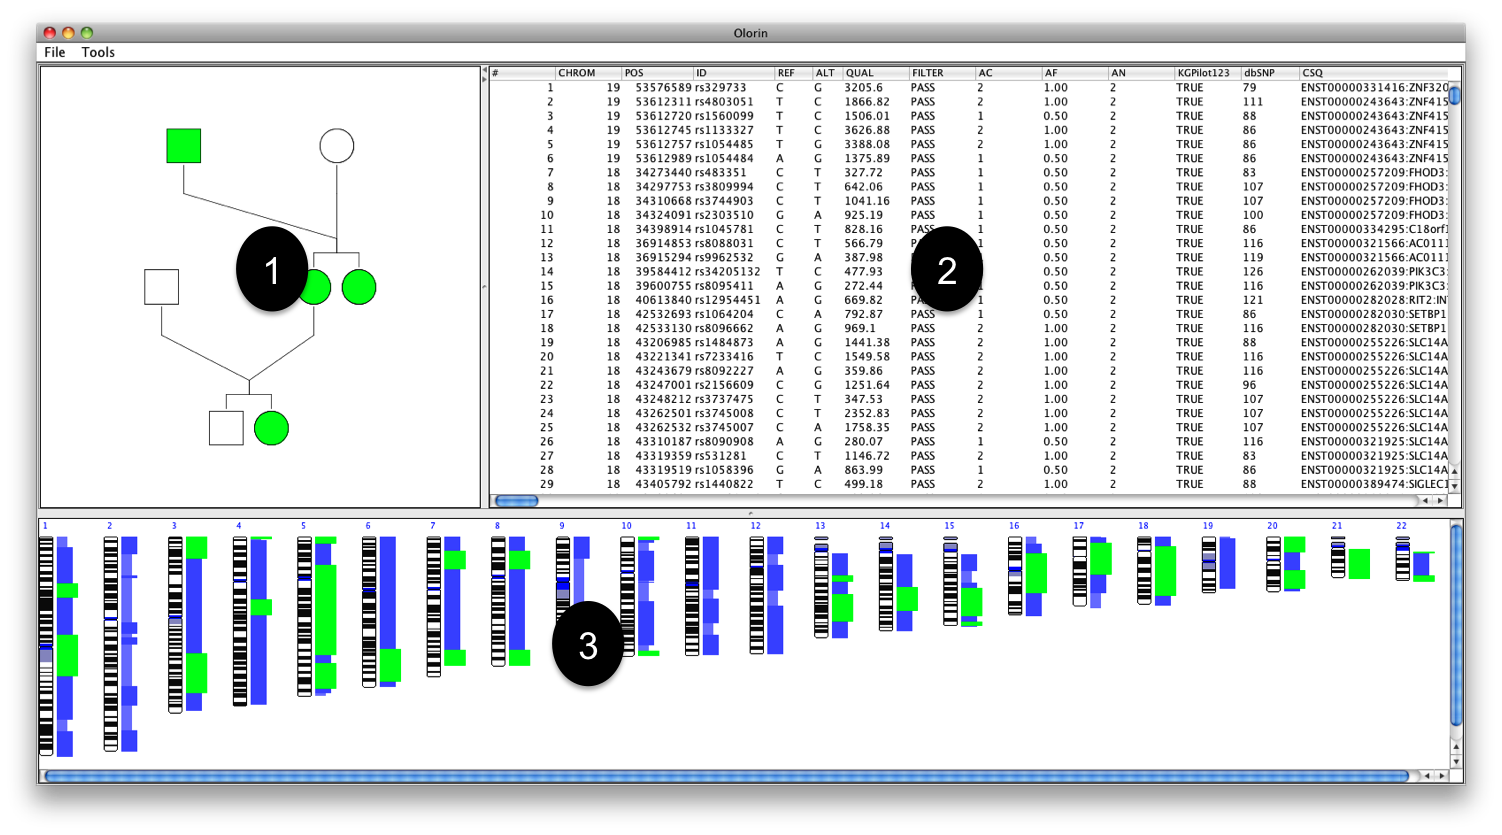
\includegraphics[scale=0.5]{olorin_main}
	\caption{The Olorin user interface.}
	\label{main}
\end{figure}
\begin{enumerate}[(a)]
	\item{The pedigree panel}
		\begin{itemize}
			\item{The pedigree panel automatically draws an interactive pedigree from the information contained in the \texttt{.ped} file.}
			\item{More information about each individuals in the pedigree can be obtained by hovering a mouse over any node to display the individual, maternal and paternal IDs and the VCF status of the node.}
			\item{Individuals in the pedigree which are male are drawn as squares and females as circles.}
			\item{Affected individuals in the pedigree are shown using filled symbols and unaffected individuals are unfilled.}
			\item{To select or unselect any individual in the pedigree simply click on the node in the pedigree, selected individuals are shown highlighted in green.}
			\item{You can zoom in and out of larger pedigrees using the popup menu displayed on right clicking or using your mouse scrolling wheel.}
			\item{The pedigree panel can be fully expanded to the full X or Y dimension of the Olorin window using the clickable expand arrows found in the each of the panel dividers.}
		\end{itemize}
	\item{Variant counter}
		\begin{itemize}
			\item{The counter displays both the total number of variants present in all the identified genomic regions for the filtering mode selected and the number of variants currently shown in the variant panel after all the filtering options have been applied.}
		\end{itemize}
	\item{Filtering modes}
		\begin{itemize}
			\item{Any individual mode:} In this mode Olorin will display variants in the variant table which are polymorphic in any one of the individuals present in the \texttt{VCF} file in the identified genomic regions.
			\item{Selected individuals mode:} In this mode Olorin will display variants in the variant table which are polymorphic is all of the user selected individuals in the identified genomic regions.
			\item{All individuals mode:} In this mode Olorin will display variants in the variant table which are polymorphic in all of the individuals present in the \texttt{VCF} file in the identified genomic regions.
		\end{itemize}
	\item{Find Segments Button}
		\begin{itemize}
			\item{The Find Segments button launches the initial filtering dialog.}
		\end{itemize}
		\item{Update Segments Button}
		\begin{itemize}
			\item{The Update Segments Button allows you to refresh the segments displayed in both the variants panel and the genome wide sharing panel after the individuals selected in the pedigree has been changed.} 
		\end{itemize}		
	\item{The filtering panel}
		\begin{itemize}
			\item{Dynamic filtering tools are generated for each of the selected INFO and CSQ fields in the VCF.}
			\item{Depending on the data type different tools are created:}
				\begin{itemize}
					\item{string - Free text search box}
					\item{int/float - Cutoff generator}
					\item{flag - true/false checkbox}
				\end{itemize}
		\end{itemize}
	\item{The variants panel}
		\begin{itemize}
			\item{The variants panel displays all the variants from the \texttt{VCF} which pass the filtering criteria that has been set.}
			\item{The table of variants can be sorted on any of the columns by simply clicking on the column heading.}
			\item{The variants panel can be fully expanded to the full X or Y dimension of the Olorin window using the clickable expand arrows found in the each of the panel dividers.}
		\end{itemize}		
	\item{The genome wide sharing panel}
		\begin{itemize}
			\item{The genome wide sharing plots show all the regions shared by the currently selected individuals across the genome.}
			\item{The shade and height of each region reflects the number of chromosomes shared at that position across in genome.}
			\item{Regions which are greater than or equal to the minimum matching chromosomes threshold set by the user are coloured in green.}
			\item{The genome wide sharing panel can be fully expanded to the full X or Y dimension of the Olorin window using the clickable expand arrows found in the each of the panel dividers.}
		\end{itemize}
\end{enumerate}

\section{Tutorial}
The easiest way to learn how to use Olorin is to test it with the included sample dataset

The sample dataset in the \texttt{example\_data} folder contains haplotypes from MERLIN and sequenced variants for a single chromosome (chromosome 22) belonging to a pedigree containing 13 members 9 of which are affected.

You should be able to launch the program by double- clicking the Olorin icon.

\subsection{Opening a directory}
Open the data directory by selecting Open directory from the File menu and select the directory where you�ve put the \texttt{example\_data} directory.

\subsection{Selecting individuals}
To find the shared segments between a set of individuals in a pedigree you first need to select the individuals.\\

To select an individual in Olorin you simply need to click on the individual in the pedigree, once an individual is selected they will be highlighted in green.\\

Be sure to always select at least one individual that has sequence data, otherwise Olorin will not allow you to search for shared segments.

Once all the desired individuals have been highlighted, select the `Find Segments' button in filtering panel, an initial filtering window will then be launched.

\subsection{General options}
	This first tab lets you set the minimum number of chromosomes that must be shared across segments using a sliding bar in the window.\\

	If your VCF file does not contain population frequencies for filtering out common variants it is possible to load frequencies from a separate file and apply a cut off to all selected variants.

	There is an example frequency file included in the example data, to use it click the `filter variants by frequency' button and select the \texttt{example.22.frq.gz} file from your \texttt{example\_data} directory.
	
	You can then change the frequency cut-off by typing a new value in the text box.

\subsection{Info field options}
	 This tab allows you to select the additional information from the \texttt{INFO} field of the \texttt{VCF} you wish to display in the table of shared variants. 
	 
	 Simply tick each field you would like to display in the variants table following initial filtering.
	 
\subsection{Consequence options}
	If your \texttt{VCF} file contains consequence data in the \texttt{INFO} field as the example data does, you can use this tab to select the consequence information you wish to display for each variant.


Once you are happy with all the initial filtering options just click the \texttt{Go} button to get your results. The initial filtering process may take some time if there are a large number of shared variants, such a case is common when looking for shared segments in small pedigrees.

\subsection{Real time filtering}

	When the initial filtering process is complete the main Olorin interface will be updated to show all the shared variants that have been found. The filtering panel should also now display real-time filters for all of the selected additional information columns and the genomewide sharing panel will also now display a plot of the all the regions shared by the currently selected individuals across the genome.

\subsection{Exporting Segment data}
To save details of all the segments shared between the currently selected individuals in a tab separated file select \texttt{Export Segments} from the \texttt{File} menu, then simply enter a file name and location for the segments to be saved to.

\subsection{Export Variants}
To save all the variants currently in the variants panel in a tab separated file select \texttt{Export Variants} from the \texttt{File} menu, then simply enter a file name and location for the variants to be saved to.

\subsection{Save the genome wide sharing plot}
To save the genome wide sharing plot as a \texttt{.png} select \texttt{Save plot} from the \texttt{Tools} menu and enter a file name and location for the plot to be saved to.

%\section{User settings}
%In order to make it easier to apply the same set of filters to a number of datasets users can save their filtering settings to a file. Once a pedigree has been loaded and segments have been found the user can select the \texttt{Save Filtering Settings} from the \texttt{File} menu. This operation will generate a file containing details of the currently selected results columns and the filtering settings. The user can load a set of preferences at any point after a pedigree has been load by selecting \texttt{Load Filtering Settings} from the \texttt{File} menu.

\section{Most damaging consequence}	
	When there is more than one consequence for a variant only the details of the most damaging effect will be displayed. If however you wish to view all the consequences you can do so by simply clicking on the number in \texttt{Total Number of Effects} column, as this will create a popup containing details of all the consequences for the variant.
	
	The most damaging consequence is selected by scoring each consequence on the following scale and selecting the first consequence with the highest score:\\

\begin{tabular}{ l c }
UPSTREAM & 1\\
DOWNSTREAM & 1\\
INTRONIC & 1\\
INTERGENIC & 1\\	
5PRIME UTR	& 2\\
3PRIME UTR	& 2\\
SYNONYMOUS CODING & 2\\
WITHIN MATURE miRNA & 2\\
STOP GAINED & 3\\
STOP LOST & 3\\
SPLICE SITE	& 3\\
COMPLEX INDEL & 3\\
FRAMESHIFT CODING & 3\\
ESSENTIAL SPLICE SITE & 3\\
NON SYNONYMOUS CODING & 3\\
\end{tabular}

\section{Troubleshooting}
  \subsection{Loading data}
    \begin{itemize}
    
    \item{\bf Why can Olorin not find my VCF index?}\\
    Where a VCF file is named in the following way:\\
    \texttt{example.vcf.gz}\\
    Olorin expects the VCF index file to be named:\\
    \texttt{example.vcf.gz.tbi}\\
    
    \item{\bf What should I do if Olorin has problems fetching variants from the VCF?}\\
    First test that your VCF file was successfully indexed, you can do this on the command line using tabix and the following command:\\
    \texttt{tabix example.vcf.gz 1:0-1000000}\\
    This command should print out all the variants in the first megabase of chromosome one in your VCF.
    Try this command on a region of the genome that you know contains variants, if this does not work then try indexing your VCF again.\\    
    If this does not help then you should also check that your VCF is in a valid format. You can check if your VCF is valid using VCFtools (\href{http://vcftools.sourceforge.net/docs.html\#validator}{http://vcftools.sourceforge.net/docs.html\#validator}).
    \item{\bf What options does MERLIN require to produce output for Olorin?}
    Olorin requires the \texttt{.flow} files to be in the horizontal format for outputting haplotypes, MERLIN should therefore be run using the \texttt{--horizontal} flag.
  \end{itemize}

\subsection{Display}
  \begin{itemize}
    \item{\bf How can I make the genome wide ideogram plot larger?}\\
    You can use the clickable expanding arrows found in each of the panel dividers allow each of the panels to be fully expanded to the full X or Y dimension of the Olorin window
    \item{\bf How can I identify the sample name of a node in the pedigree?}
    Holding the pointer over the point of interest will show which sample corresponds to that node.
  \end{itemize}
  
\subsection{Other}
  \begin{itemize}
    \item{\bf What do I do if Evoker runs out of memory?}
    If Olorin needs more memory to load a data set then users can launch the program with additional memory from the command line by issuing the following command (increasing the -Xmx value as necessary):
    java -Xmx1024m -jar Evoker.jar
  \end{itemize}

\section{Resources}
\begin{itemize}
  \item{MERLIN:}\\
  \href{http://www.sph.umich.edu/csg/abecasis/Merlin/}{http://www.sph.umich.edu/csg/abecasis/Merlin/}
  \item{Flow file format:}\\
  \href{http://www.sph.umich.edu/csg/abecasis/Merlin/tour/haplotyping.html}{http://www.sph.umich.edu/csg/abecasis/Merlin/tour/haplotyping.html}
  \item{Map file format:}\\
  \href{http://pngu.mgh.harvard.edu/~purcell/plink/data.shtml#map}{http://pngu.mgh.harvard.edu/~purcell/plink/data.shtml\#map}
  \item{Ped file format:}\\
  \href{http://pngu.mgh.harvard.edu/~purcell/plink/data.shtml#ped}{http://pngu.mgh.harvard.edu/~purcell/plink/data.shtml\#ped}
  \item{VCF file format:}\\
  \href{http://www.1000genomes.org/node/101}{http://www.1000genomes.org/node/101}
  \item{tabix and bgzip:}\\
  \href{http://sourceforge.net/projects/samtools/files/tabix/}{http://sourceforge.net/projects/samtools/files/tabix/}
  \item{VCFtools:}\\
  \href{http://vcftools.sourceforge.net/}{http://vcftools.sourceforge.net/}
\end{itemize}

\end{document}